
\documentclass{article}

\usepackage{fullpage,latexsym,picinpar,amsmath,amsfonts,graphicx}



\setlength{\evensidemargin}{0.1in}
\setlength{\oddsidemargin}{0.1in}
\setlength{\textwidth}{6.6in}
\setlength{\topmargin}{0.0in}
\setlength{\textheight}{8.7in}
\setlength{\headheight}{0in}
\setlength{\headsep}{0in}
\setlength{\topsep}{0in}
\setlength{\itemsep}{0in}
\renewcommand{\baselinestretch}{1.1}
\parskip=0.080in

\newcommand{\parend}[1]{{\left( #1  \right) }}
\newcommand{\spparend}[1]{{\left(\, #1  \,\right) }}
\newcommand{\angled}[1]{{\left\langle #1  \right\rangle }}
\newcommand{\brackd}[1]{{\left[ #1  \right] }}
\newcommand{\spbrackd}[1]{{\left[\, #1  \,\right] }}
\newcommand{\braced}[1]{{\left\{ #1  \right\} }}
\newcommand{\leftbraced}[1]{{\left\{ #1  \right. }}
\newcommand{\floor}[1]{{\left\lfloor #1\right\rfloor}}
\newcommand{\ceiling}[1]{{\left\lceil #1\right\rceil}}
\newcommand{\barred}[1]{{\left|#1\right|}}
\newcommand{\doublebarred}[1]{{\left|\left|#1\right|\right|}}
\newcommand{\spaced}[1]{{\, #1\, }}
\newcommand{\suchthat}{{\spaced{|}}}
\newcommand{\numof}{{\sharp}}

\newcommand{\half}{{\textstyle\frac{1}{2}}}
\newcommand{\elevenhalves}{{\textstyle\frac{11}{2}}}
\newcommand{\onethird}{{\textstyle\frac{1}{3}}}
\newcommand{\sixteenthirds}{{\textstyle\frac{16}{3}}}
\newcommand{\twentytwothirds}{{\textstyle\frac{22}{3}}}
\newcommand{\onefifth}{{\textstyle\frac{1}{5}}}
\newcommand{\threefifths}{{\textstyle\frac{3}{5}}}
\newcommand{\sixfifths}{{\textstyle\frac{6}{5}}}
\newcommand{\eightfifths}{{\textstyle\frac{8}{5}}}
\newcommand{\sixteenfifths}{{\textstyle\frac{16}{5}}}
\newcommand{\eightteenfifths}{{\textstyle\frac{18}{5}}}
\newcommand{\threetenths}{{\textstyle\frac{3}{10}}}
\newcommand{\twentysixfifteenths}{{\textstyle\frac{26}{15}}}
\newcommand{\fisefiftieths}{{\textstyle\frac{57}{50}}}
\newcommand{\ftwotfifths}{{\textstyle\frac{42}{25}}}
\newcommand{\fotwontwfifths}{{\textstyle\frac{42}{125}}}
\newcommand{\eithontwfifths}{{\textstyle\frac{83}{125}}}

\newcommand{\veps}{{\varepsilon}}
\newcommand{\Sigmastar}{{\Sigma^\ast}}

\newcounter{exnum}[section]
\newenvironment{problem}{{\vskip 0.1in
   \noindent \bf Problem\addtocounter{exnum}{1}~\arabic{exnum}.}}{\vskip 0.1in}

\newtheorem{theorem}{Theorem}
\newtheorem{definition}{Definition}
\newtheorem{corollary}{Corollary}
\newtheorem{lemma}{Lemma}
\newtheorem{fact}{Fact}
\newtheorem{claim}{Claim}

\newenvironment{proof}{{\it Proof:\/}}{$\Box$\vskip 0.1in}

\newcommand{\emparagraph}[1]{{\smallskip\noindent{\em #1\/}}}

\newcommand{\assign}{{\,\gets\,}}

%%%%%%%%%%%%%%%%%%%%%%%%%%%%%%%%%%%%%%%%%%%%%%%%%%%%%%%%%%%%%%%%%%%%%%%%%%%%%%%%%%%
%%%%%%%%%%%  LETTERS 
%%%%%%%%%%%%%%%%%%%%%%%%%%%%%%%%%%%%%%%%%%%%%%%%%%%%%%%%%%%%%%%%%%%%%%%%%%%%%%%%%%%

\newcommand{\barx}{{\bar x}}
\newcommand{\bary}{{\bar y}}
\newcommand{\barz}{{\bar z}}
\newcommand{\bart}{{\bar t}}

\newcommand{\bfP}{{\bf{P}}}

%%%%%%%%%%%%%%%%%%%%%%%%%%%%%%%%%%%%%%%%%%%%%%%%%%%%%%%%%%%%%%%%%%%%%%%%%%%%%%%%%%%
%%%%%%%%%%%%%%%%%%%%%%%%%%%%%%%%%%%%%%%%%%%%%%%%%%%%%%%%%%%%%%%%%%%%%%%%%%%%%%%%%%%
                                                                                  
\newcommand{\threehalfs}{\mbox{$\frac{3}{2}$}}   
\newcommand{\domino}[2]{\left[\frac{#1}{#2}\right]}  

%%%%%%%%%%%% complexity classes

\newcommand{\PP}{\mathbb{P}}
\newcommand{\NP}{\mathbb{NP}}
\newcommand{\PSPACE}{\mathbb{PSPACE}}
\newcommand{\coNP}{\textrm{co}\mathbb{NP}}
\newcommand{\DLOG}{\mathbb{L}}
\newcommand{\NLOG}{\mathbb{NL}}
\newcommand{\NL}{\mathbb{NL}}

%%%%%%%%%%% decision problems

\newcommand{\PCP}{\sc{PCP}}
\newcommand{\Path}{\sc{Path}}
\newcommand{\GenGeo}{\sc{Generalized Geography}}

\newcommand{\malytm}{{\mbox{\tiny TM}}}
\newcommand{\malycfg}{{\mbox{\tiny CFG}}}
\newcommand{\Atm}{\mbox{\rm A}_\malytm}
\newcommand{\complAtm}{{\overline{\mbox{\rm A}}}_\malytm}
\newcommand{\AllCFG}{{\mbox{\sc All}}_\malycfg}
\newcommand{\complAllCFG}{{\overline{\mbox{\sc All}}}_\malycfg}
\newcommand{\complL}{{\bar L}}
\newcommand{\TQBF}{\mbox{\sc TQBF}}
\newcommand{\SAT}{\mbox{\sc SAT}}

%%%%%%%%%%%%%%%%%%%%%%%%%%%%%%%%%%%%%%%%%%%%%%%%%%%%%%%%%%%%%%%%%%%%%%%%%%%%%%%%%%%
%%%%%%%%%%%%%%% for homeworks
%%%%%%%%%%%%%%%%%%%%%%%%%%%%%%%%%%%%%%%%%%%%%%%%%%%%%%%%%%%%%%%%%%%%%%%%%%%%%%%%%%%

\newcommand{\student}[2]{%
{\noindent\Large{ \emph{#1} SID {#2} } \hfill} \vskip 0.1in}

\newcommand{\assignment}[1]{\medskip\centerline{\large\bf CS 111 ASSIGNMENT {#1}}}

\newcommand{\duedate}[1]{{\centerline{due {#1}\medskip}}}     

\newcounter{problemnumber}                                                                                 


\newcounter{solutionnumber}

\newenvironment{solution}{{\vskip 0.1in \noindent
             \bf Solution~\addtocounter{solutionnumber}{1}\arabic{solutionnumber}:}}
				{\ \newline\smallskip\lineacross\smallskip}

\newcommand{\lineacross}{\noindent\mbox{}\hrulefill\mbox{}}

\newcommand{\decproblem}[3]{%
\medskip
\noindent
\begin{list}{\hfill}{\setlength{\labelsep}{0in}
                       \setlength{\topsep}{0in}
                       \setlength{\partopsep}{0in}
                       \setlength{\leftmargin}{0in}
                       \setlength{\listparindent}{0in}
                       \setlength{\labelwidth}{0.5in}
                       \setlength{\itemindent}{0in}
                       \setlength{\itemsep}{0in}
                     }
\item{{{\sc{#1}}:}}
                \begin{list}{\hfill}{\setlength{\labelsep}{0.1in}
                       \setlength{\topsep}{0in}
                       \setlength{\partopsep}{0in}
                       \setlength{\leftmargin}{0.5in}
                       \setlength{\labelwidth}{0.5in}
                       \setlength{\listparindent}{0in}
                       \setlength{\itemindent}{0in}
                       \setlength{\itemsep}{0in}
                       }
                \item{{\em Instance:\ }}{#2}
                \item{{\em Query:\ }}{#3}
                \end{list}
\end{list}
\medskip
}

%%%%%%%%%%%%%%%%%%%%%%%%%%%%%%%%%%%%%%%%%%%%%%%%%%%%%%%%%%%%%%%%%%%%%%%%%%%%%%%%%%%
%%%%%%%%%%%%% for quizzes
%%%%%%%%%%%%%%%%%%%%%%%%%%%%%%%%%%%%%%%%%%%%%%%%%%%%%%%%%%%%%%%%%%%%%%%%%%%%%%%%%%%

\newcommand{\quizheader}{ {\large NAME: \hskip 3in SID:\hfill}
                                \newline\lineacross \medskip }

%\newcommand{\namespace}{ {\large NAME: \hskip 3in SID:\hfill}
%                               \newline\lineacross \medskip }

%%%%%%%%%%%%%%%%%%%%%%%%%%%%%%%%%%%%%%%%%%%%%%%%%%%%%%%%%%%%%%%%%%%%%%%%%%%%%%%%%%%
%%%%%%%%%%%%% for final
%%%%%%%%%%%%%%%%%%%%%%%%%%%%%%%%%%%%%%%%%%%%%%%%%%%%%%%%%%%%%%%%%%%%%%%%%%%%%%%%%%%

\newcommand{\namespace}{\noindent{\Large NAME: \hfill SID:\hskip 1.5in\ }\\\medskip\noindent\mbox{}\hrulefill\mbox{}}




\newcommand{\hwduedate}{{}}

\begin{document}

\centerline{\large \bf CS111 ASSIGNMENT 5}

\vskip 0.25in

%%%%%%%%%%%%%%%%
% problem 1

\begin{problem}
Determine whether the two graphs below are planar or not.
To show planarity, give a planar embedding.
To show that a graph is not planar, use Kuratowski's theorem.

\bigskip

\begin{center}
{\large Graph $H$:\ }
\begin{minipage}{2.1in}
        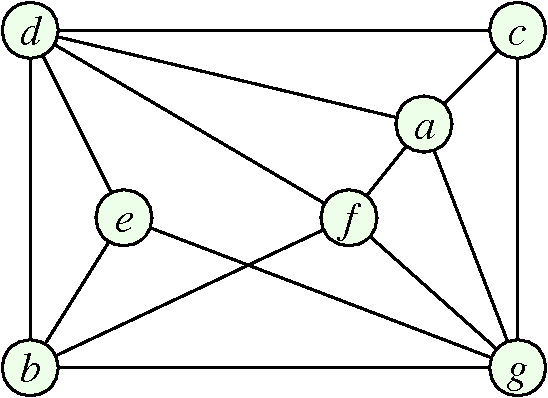
\includegraphics[width=2in]{planar_graphH_hw5.pdf}
\end{minipage}
\hfill
{\large Graph $G$:\ }
\begin{minipage}{2.4in}
        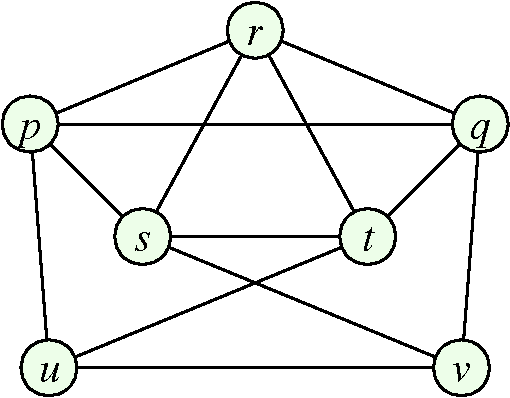
\includegraphics[width=1.8in]{planar_graphG_hw5.pdf}
\end{minipage}
\end{center}
\end{problem}

%%%%%%%%%%%%%%%%%
% solution 1

\begin{solution}
	\\ For graph H, you can make a planar embedding by moving vertex $e$, therefore, it is planar.
	\\ 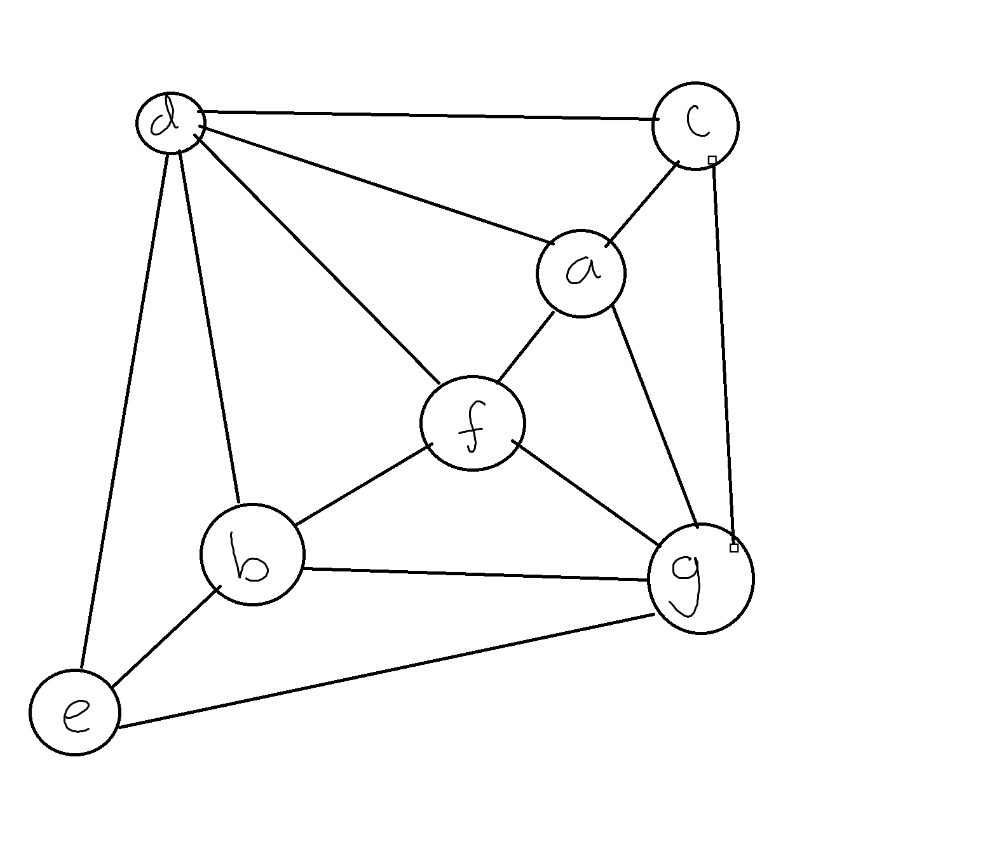
\includegraphics[scale=0.2]{h.png}
	\\ For graph G, we can find a subgraph that is homeomorphic to $k_{3,3}$, therefore, according to Kuratowski's theorem, it is not planar.
	\\ 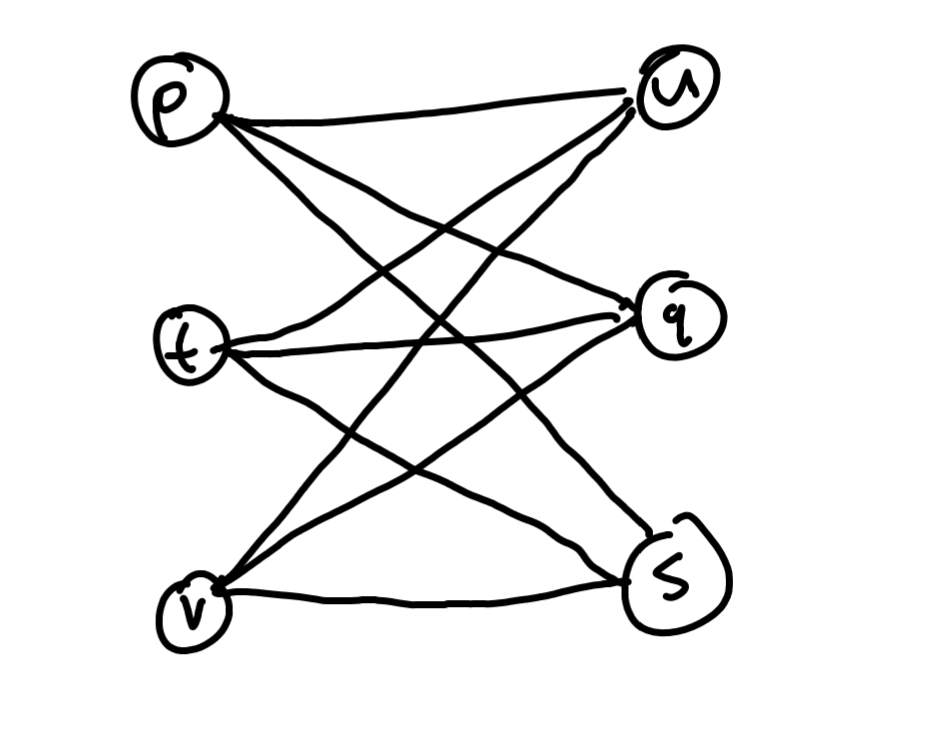
\includegraphics[scale=0.2]{g.png}
\end{solution}



%%%%%%%%%%%%%%%%%%%%%%%%%%%%
\newpage
\vskip 0.25in

\begin{problem}
(a) For each degree sequence below, determine whether there is a graph with $6$ vertices where vertices have
these degrees. If a graph exists, (i) draw it, (ii) find the chromatic number and justify. If it doesn't, justify that it doesn't exist.

\noindent Note. To give a justification for the chromatic number, you need to give a coloring and explain why it's not possible to use fewer colors.
%
%
\begin{description}\setlength{\itemsep}{-3pt}
	\item{(a1)} $5, 4, 4, 3, 3, 1$. 
	\item{(a2)} $5, 4, 3, 2, 2, 1$.
	\item{(a3)} $4, 4, 4, 3, 3, 2$.
\end{description}

\noindent (b) For each degree sequence below, determine whether there is a planar graph with $6$ vertices where vertices have
these degrees. If a graph exists, (i) draw it, (ii) find the chromatic number and justify. If it doesn't, justify that it doesn't exist.

% 
%
\begin{description}\setlength{\itemsep}{-3pt}
	\item{(b1)} $5, 5, 4, 4, 4, 2$.
	\item{(b2)} $3, 3, 3, 3, 3, 3$.
\end{description}
\end{problem}

\newpage
\begin{solution} 
	\\
	a1)  This graph does exist. Its chromatic number is 4. You can color it with 4 colors, but cannot color it with 3. This is because there are two cliques of four vertices: on the picture, it is the vertices labeled 3, 4, 5.
	\\ 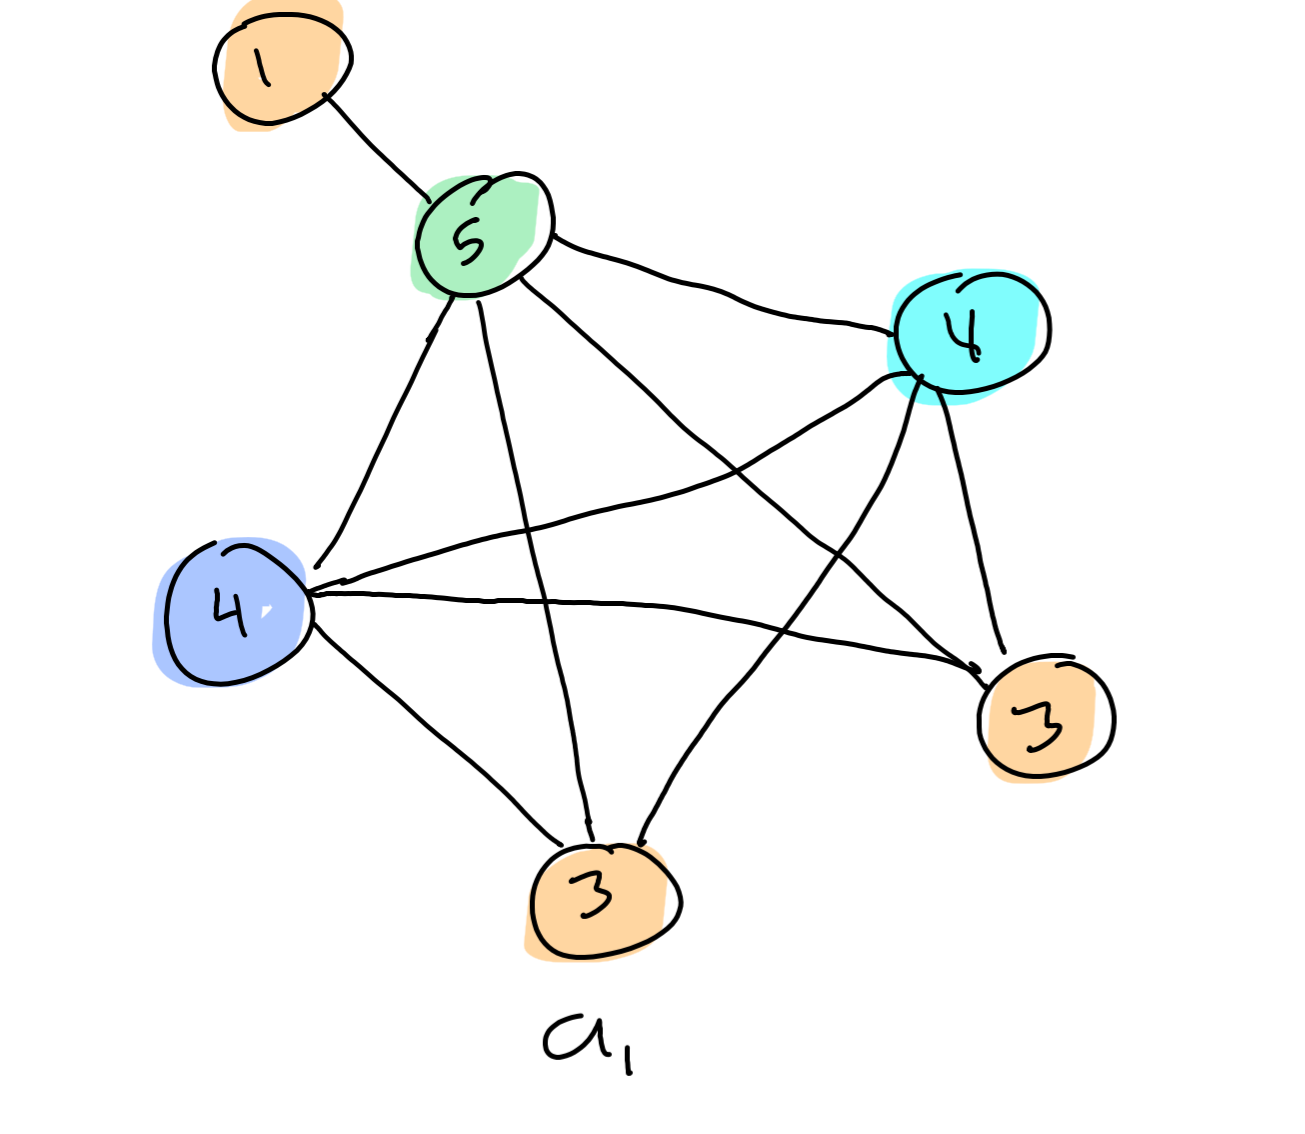
\includegraphics[scale=0.4]{a1.png}
	\\
	a2) This graph doesn't exist because the sum of degrees is not even. This violates the handshake lemma.
	\\
	a3) This graph does exist. Its chromatic number is 3. It cannot be colored with 2 colors because there is a clique of 3: the three vertices labeled 4.
	\\ 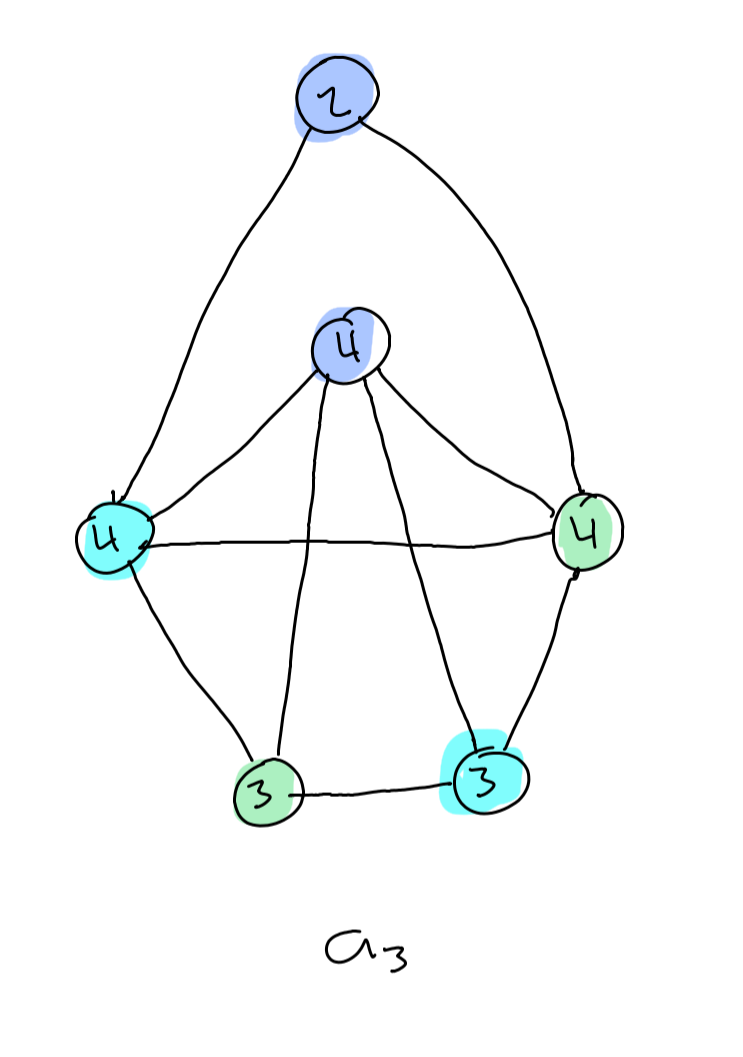
\includegraphics[scale=0.5]{a3.png}
	\\\\\\\\\\
	b1) This planar graph does not exist. When you draw the graph, you will get a graph that has a subgraph of k5 when you remove vertex 2. According to Kuratowski's theorem, this graph is not planar.
	\\ 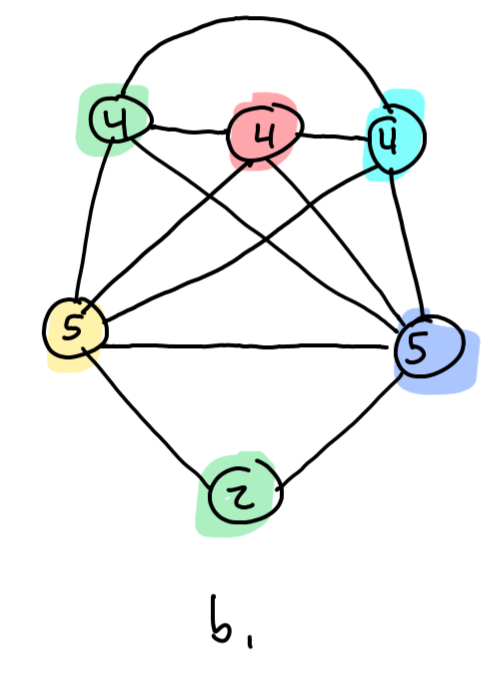
\includegraphics[width=3in]{b1.png}
	\\
	b2) This graph exists and its chromatic number is 4. Each vertex is connected to 3 other vertices, so the chromatic number is at least 4. According to the four color theorem, the chromatic number is at most 4. Since the chromatic number is at least 4 and at most 4, the chromatic number is 4.
	\\ 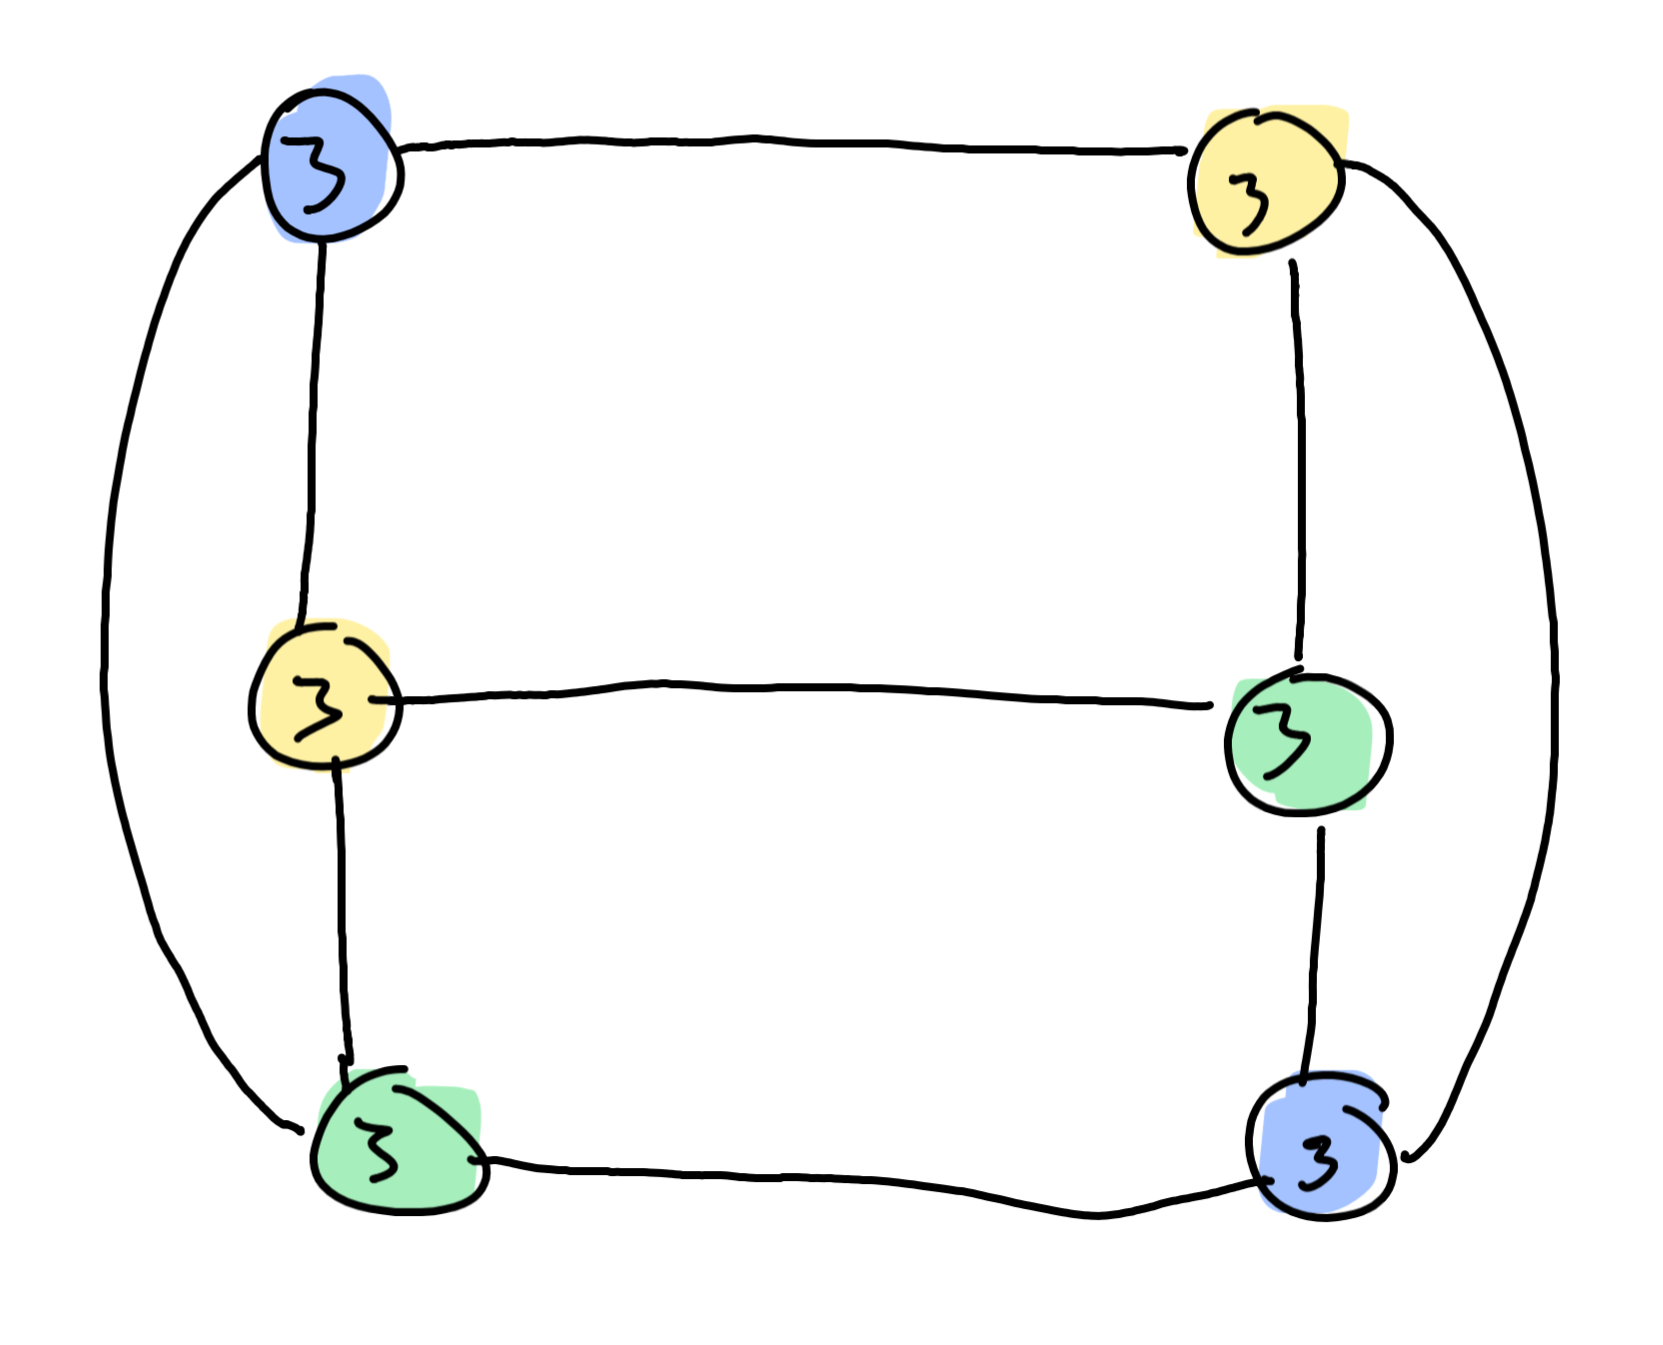
\includegraphics[width=3in]{b2.png}

\end{solution}

\vspace{0.15in}
\newpage
%%%%%%%%%%%%%%%%%%%%%%%%%%%%
\begin{problem}

a) Does the graph shown below have an Euler tour? Give a complete justification for your answer.

b) Does the graph shown below have a Hamiltonian cycle? Give a complete justification for your answer.


	\begin{center}
	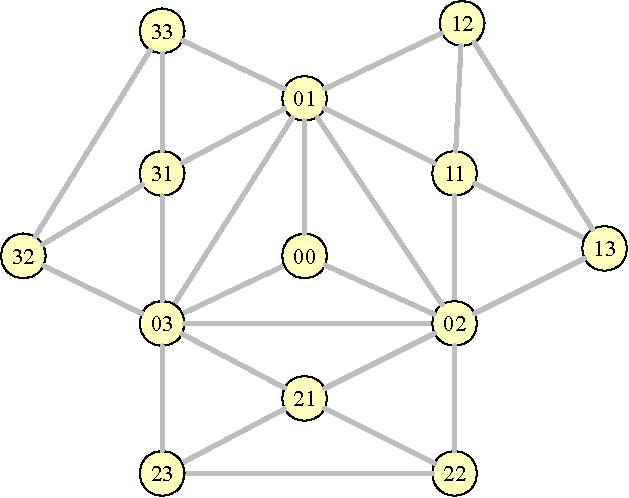
\includegraphics[width = 3in]{Ham_graph.pdf}
	\end{center}

\end{problem}

\begin{solution}\\	
	a) This graph does not have an Euler tour because there are vertices with odd degrees. For example, 33 is degree 3.
	\\
	% b) This graph has no Hamiltonian cycle. We can figure this out by using the contrapositive of Ore's theorem: If G does not have a Hamiltonian Cycle, then there is a pair of non-adjacent vertices, u and v, where $deg(u) + deg(v) < n$. Since $n=13$, and $deg(33) + deg(12) = 6 < n$, then this graph does not have a Hamiltonian cycle.
	b) This graph does not contain a Hamiltonian cycle. Imagine the graph as three rectangles surrounding a triangle. The vertices 01, 02, and 03 act like a funnel because you will have to go through them in order to move from one shape to the other. Since there are four shapes (three rectangles, one triangle), you will have to go through one of the three "funnel" vertices twice in order to get back to where you started. Therefore, this graph does not contain a Hamiltonian cycle.
	\\
\end{solution}


%%%%%%%%%%%%%%%%%%%%%%%%%%%%
\newpage

\paragraph{Academic integrity declaration.}
% The homework papers must include at the end an academic integrity declaration. This should be a short paragraph where you briefly explain 
% \emph{in your own words}  (1) whether you did the homework individually or in collaboration with a partner student (if so, provide the name), 
% and (2) whether you used any external help or resources. 

I did this homework by myself. I got help from office hours.

%%%%%%%%%%%%%%%%%%%%%%%%%%%%

% \vskip 0.1in
% \paragraph{Submission.}
% To submit the homework, you need to upload the pdf file to Gradescope. If you submit with a partner, you need
% to put two names on the assignment and submit it as a group assignment.
% Remember that only {\LaTeX} papers are accepted. 


\end{document}

